% !TEX root =  ../../../thesis.tex
\section{Motivation}\label{sec:aps:motivation}
As explained in Chapter~\ref{ch:intro}, one of the most well-studied
deformable models are AAMs~\cite{cootes2001active,matthews2004active}. In the
previous chapter (Chapter~\ref{ch:aam}), we showed that the combination of the
Simultaneous~\cite{gross2005generic} and
Alternating~\cite{papandreou2008adaptive,tzimiropoulos2012generic} inverse
compositional algorithms with powerful features can achieve very accurate and
robust performance. On the other hand, the Project-Out inverse compositional
(POIC)~\cite{matthews2004active} algorithm has a real-time complexity but is
inaccurate, which makes it unsuitable for generic settings. Therefore, AAMs
have two disadvantages:
\begin{enumerate}
  \item They are slow and inappropriate for real-time applications.
  \item By employing PCA the appearance of the object is modeled with a single multivariate normal distribution, which, as it will be shown in this chapter, restricts the fitting accuracy (Fig.~\ref{fig:gmrf}).
\end{enumerate}

Mainly due to the high complexity when using a holistic appearance
representation, many existing methods employ a part-based one. This means that
a local patch is extracted from the neighborhood around each landmark, as shown
in Sec.~\ref{sec:notation:part_based}. Among the most important part-based
deformable models are Pictorial Structures
(PS)~\cite{fischler1973representation,felzenszwalb2005pictorial,andriluka2009pictorial}, their discriminative descendant Deformable Part Model
(DPM)~\cite{felzenszwalb2010object,zhu2012face} and their extensions like
Deformable Structures~\cite{zuffi2012pictorial}. PS learn a patch expert for
each part and model the shape of the object using spring-like connections
between parts based on a tree structure. Thus, a different distribution is
assumed for each pair of parts connected with an edge, as opposed to the PCA
shape model of AAMs that assumes a single multivariate normal distribution for
all parts. The optimization aims to find a tree-based shape configuration for
which the patch experts have a minimum cost and is performed using a dynamic
programming algorithm based on the distance
transform~\cite{felzenszwalb2000efficient}. PS are successfully used for
various tasks, such as human pose estimation~\cite{yang2013articulated} and
face detection~\cite{zhu2012face,mathias2014face}. Their biggest advantage
is that they find the global optimum, thus they are not dependent neither
require initialization. The dynamic programming technique computes all the
responses for all the possible configurations of the parts and selects the one
with the minimum cost. However, in practice, PS have two important
disadvantages:
\begin{enumerate}
  \item Inference is very slow.
  \item Because the tree structure restricts too much the range of possible
  realizable shape configurations, the global optimum, even though it is the
  best solution in the span of the model, it does not always correspond to the
  shape that best describes the object in reality.
\end{enumerate}

The method proposed in this chapter takes advantage of the strengths, and
overcomes the disadvantages, of both AAMs and PS. We are motivated by the
tree-based structure of PS and we further expand on this concept. Our model can
formulate the relations between parts using any graph structure; not only
trees. From AAMs we borrow the use of the Gauss-Newton algorithm in combination
with a statistical shape model. Our weighted inverse compositional algorithm
with fixed Jacobian and Hessian provides close to real-time cost with
state-of-the-art performance. Thus, the proposed model shares characteristics
from both AAMs and PS, hence the name Active Pictorial Structures (APS).

%
\begin{figure}[!t]
  \centering
  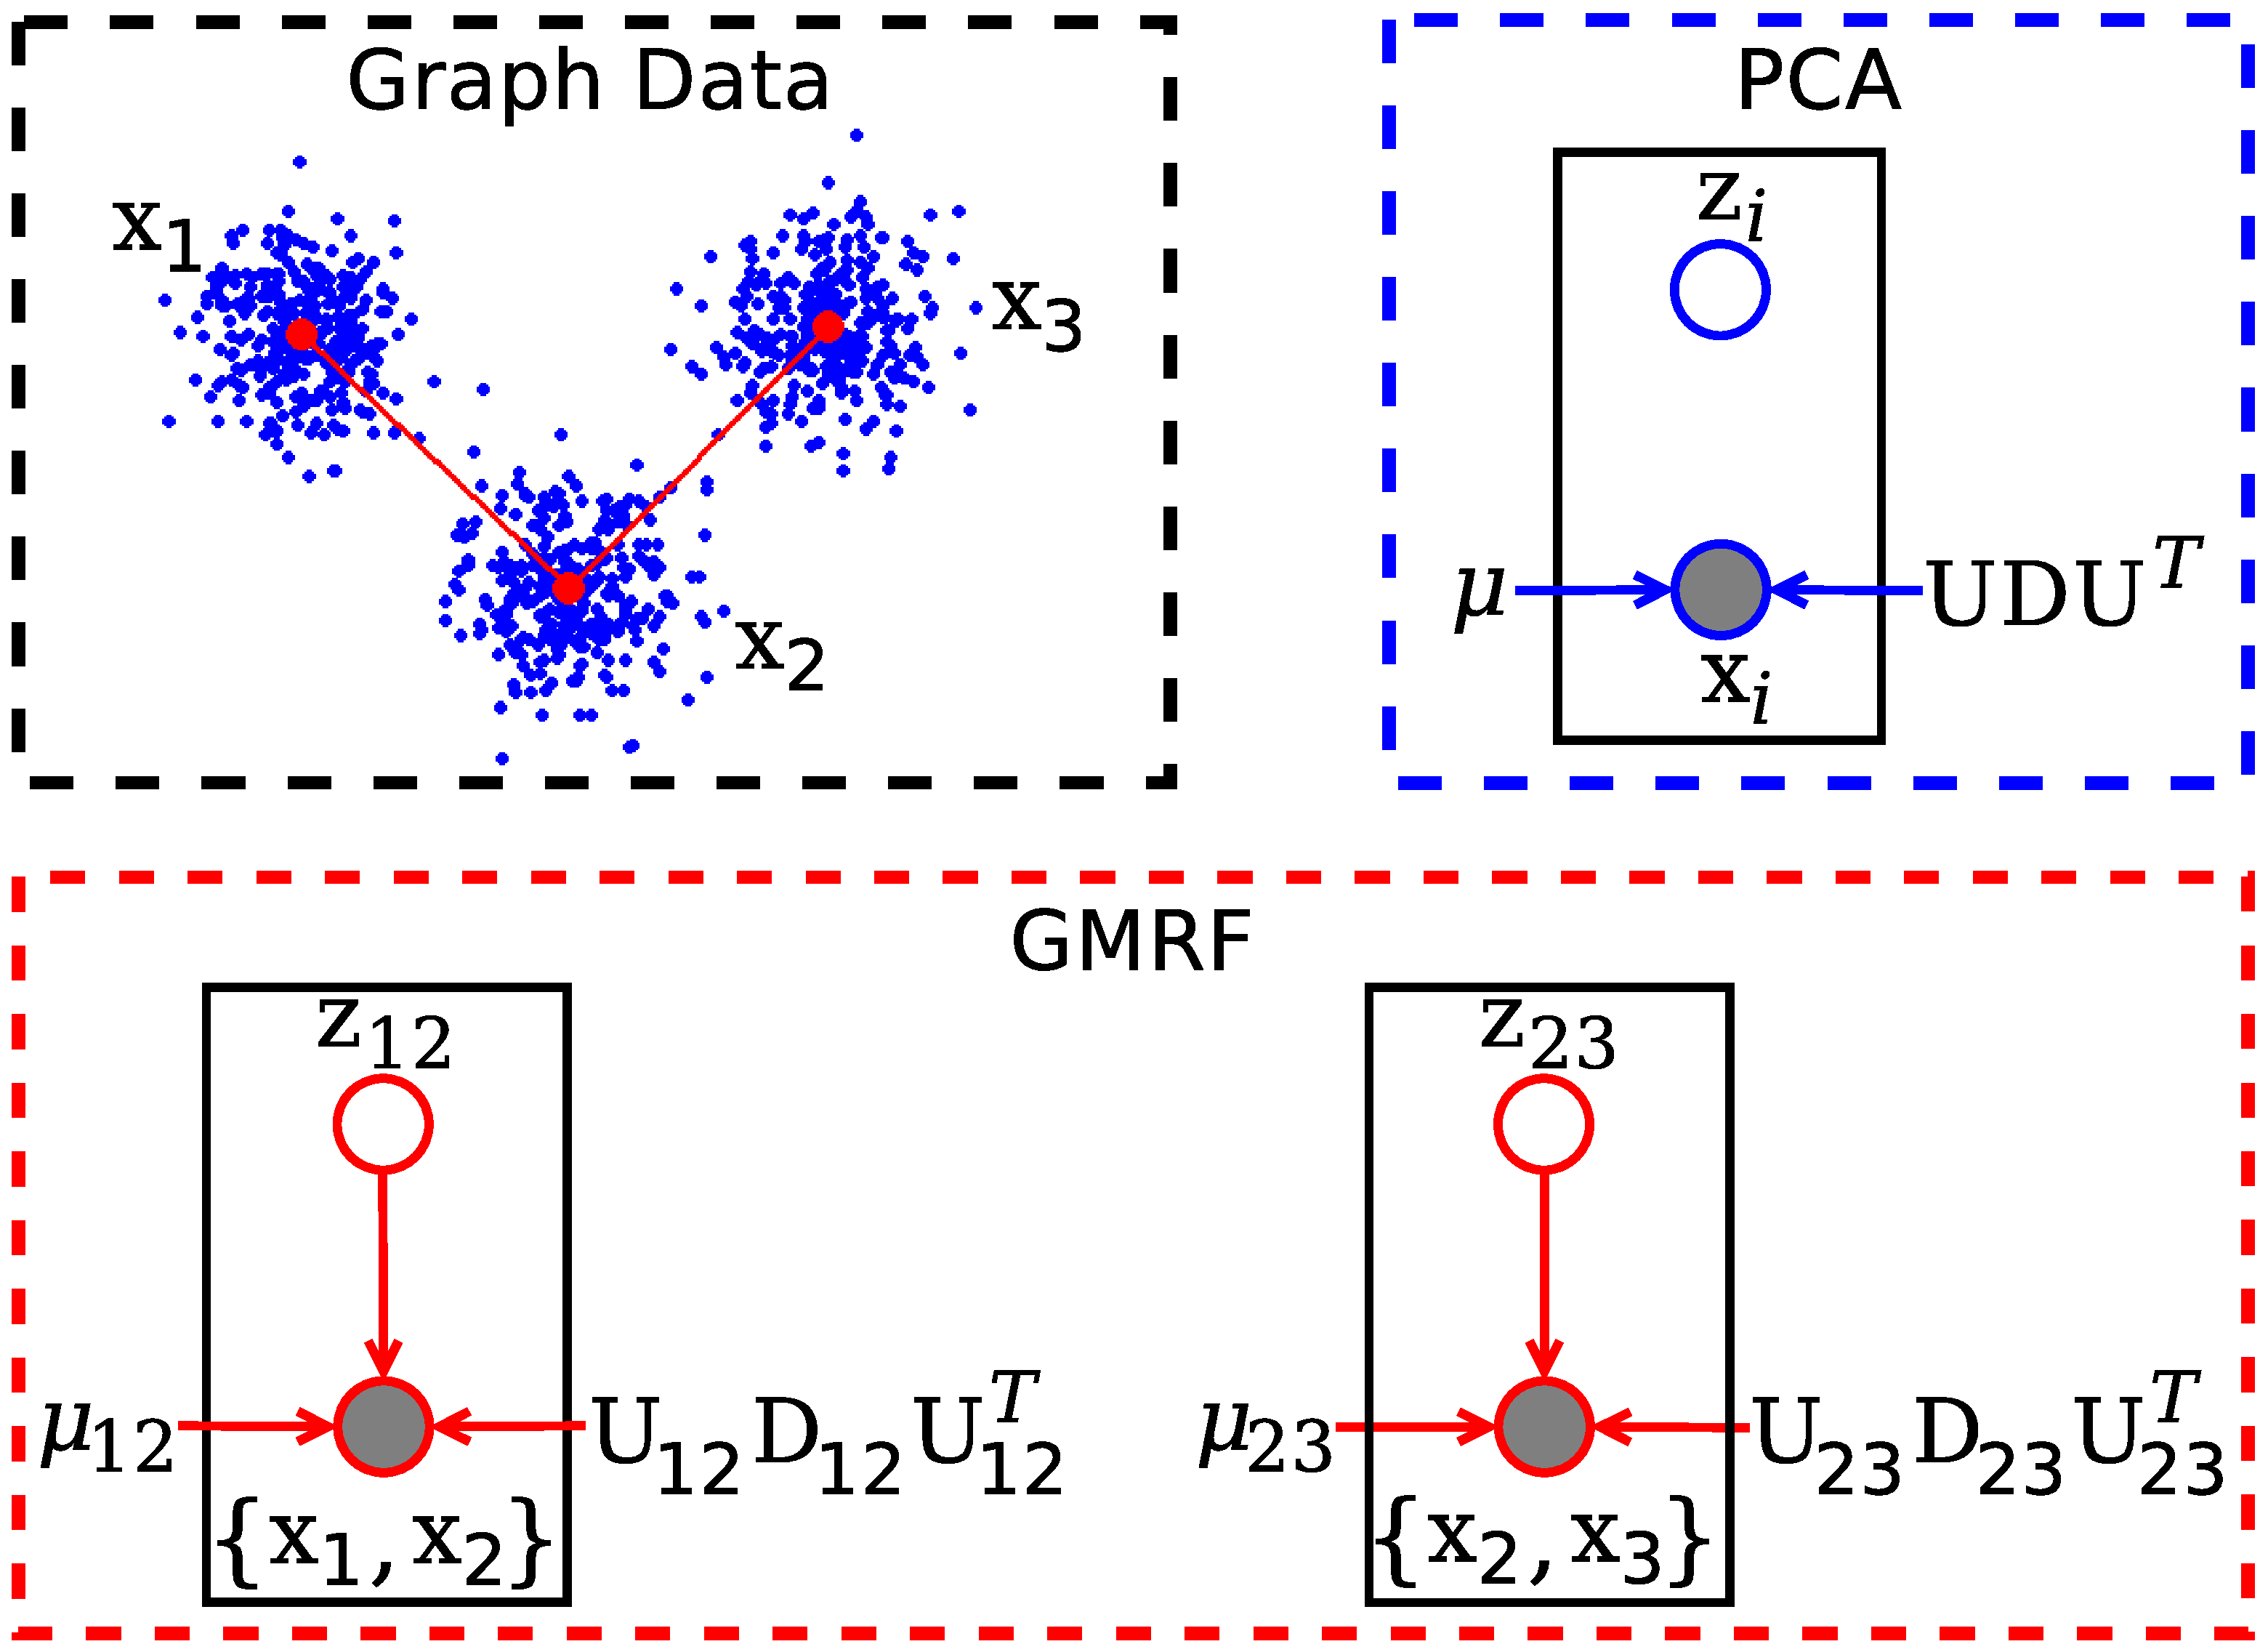
\includegraphics[width=0.5\linewidth]{figures/aps/model/model_camera_ready.eps}
  \caption{A simple visualization motivating the main idea behind APS. We
  propose to model the appearance of an object using multiple pairwise
  distributions based on the edges of a graph (GMRF) and show that this
  outperforms the commonly used PCA model under an inverse Gauss-Newton
  optimization framework.}
  \label{fig:gmrf}
\end{figure}
%

The idea of substituting the PCA shape model with a piece-wise linear model has
also been proposed for 3D facial models in~\cite{tena2011interactive}. The most
closely related method to the proposed APS is the Gauss-Newton Deformable Part
Model (GN-DPM)~\cite{tzimiropoulos2014gauss}. It is a part-based AAM that takes
advantage of the efficient inverse alternating Gauss-Newton technique proposed
in~\cite{tzimiropoulos2013optimization} and reports very accurate performance.
The two most important differences between the proposed APS and GN-DPM are
that: \emph{(i)}~APS do not model the appearance of an object using PCA but
assume a different distribution for each pair of connected parts that proves to
perform better, \emph{(ii)}~APS employ a weighted inverse compositional
algorithm with fixed Jacobian and Hessian, which is by definition at least an
order of magnitude faster than the alternating one.

In summary, the contributions of this work are:
%%%%%%%%%%%%%
\begin{itemize}
  \item The proposed model combines the advantages of PS (graph-based relations
  between parts) and AAMs (weighted inverse Gauss-Newton optimization with
  statistical shape model).
  %
  \item We show that it is more accurate to model the appearance of an object with multiple graph-based normal distributions, thus using a Gaussian Markov
  Random Field~\cite{rue2005gaussian} structure, rather than a single
  multidimensional normal distribution (PCA), as is commonly done in
  literature. We also prove that this is not beneficial for modeling an
  object's shape, because the resulting covariance matrix has high rank and the
  shape subspace has too many dimensions to be optimized. We also show that
  employing a tree structure for the shape model, as done in
  PS~\cite{felzenszwalb2005pictorial,felzenszwalb2010object,zhu2012face},
  limits the model's descriptiveness and hampers the performance.
  %
  \item We use the spring-like shape model of PS and DPM as a shape prior in
  the Gauss-Newton optimization. This deformation term makes the model more
  robust as it manages to restrict non-realistic instances of the object's
  shape.
  %
  \item We propose, to the best of our knowledge, the best performing weighted
  inverse compositional Gauss-Newton algorithm with fixed Jacobian and Hessian.
  As it will be shown, its computational cost reduces to a single matrix
  multiplication per iteration and is independent of the employed graph
  structure. We test the proposed method on the task of face alignment, because
  of the plethora of annotated facial data. However, it can also be applied to
  other objects, such as eyes, cars etc. Our experiments show that APS
  outperform the current state-of-the-art methods.
\end{itemize}
%%%%%%%%%%%%%

\noindent The content of this chapter is based on the following publication:
\begin{itemize}
  \item \textbf{E. Antonakos}, J. Alabort-i-Medina, and S. Zafeiriou.
  ``Active Pictorial Structures'',
  \emph{Proceedings of IEEE International Conference on Computer Vision and Pattern Recognition (CVPR)},
  Boston, MA, USA, pp. 5435-5444, June 2015.
\end{itemize}

The rest of the chapter is structured as follows: Section~\ref{sec:aps:method}
explains the training and fitting of the proposed method.
Section~\ref{sec:aps:exp} presents extended experimental results on the human
face and other deformable objects (eyes, cars). Finally,
Section~\ref{sec:aps:con} summarizes the outcomes of this chapter and draws
conclusions.
